\documentclass{standalone}
\usepackage{tikz}
\usetikzlibrary{patterns, positioning}

\begin{document}
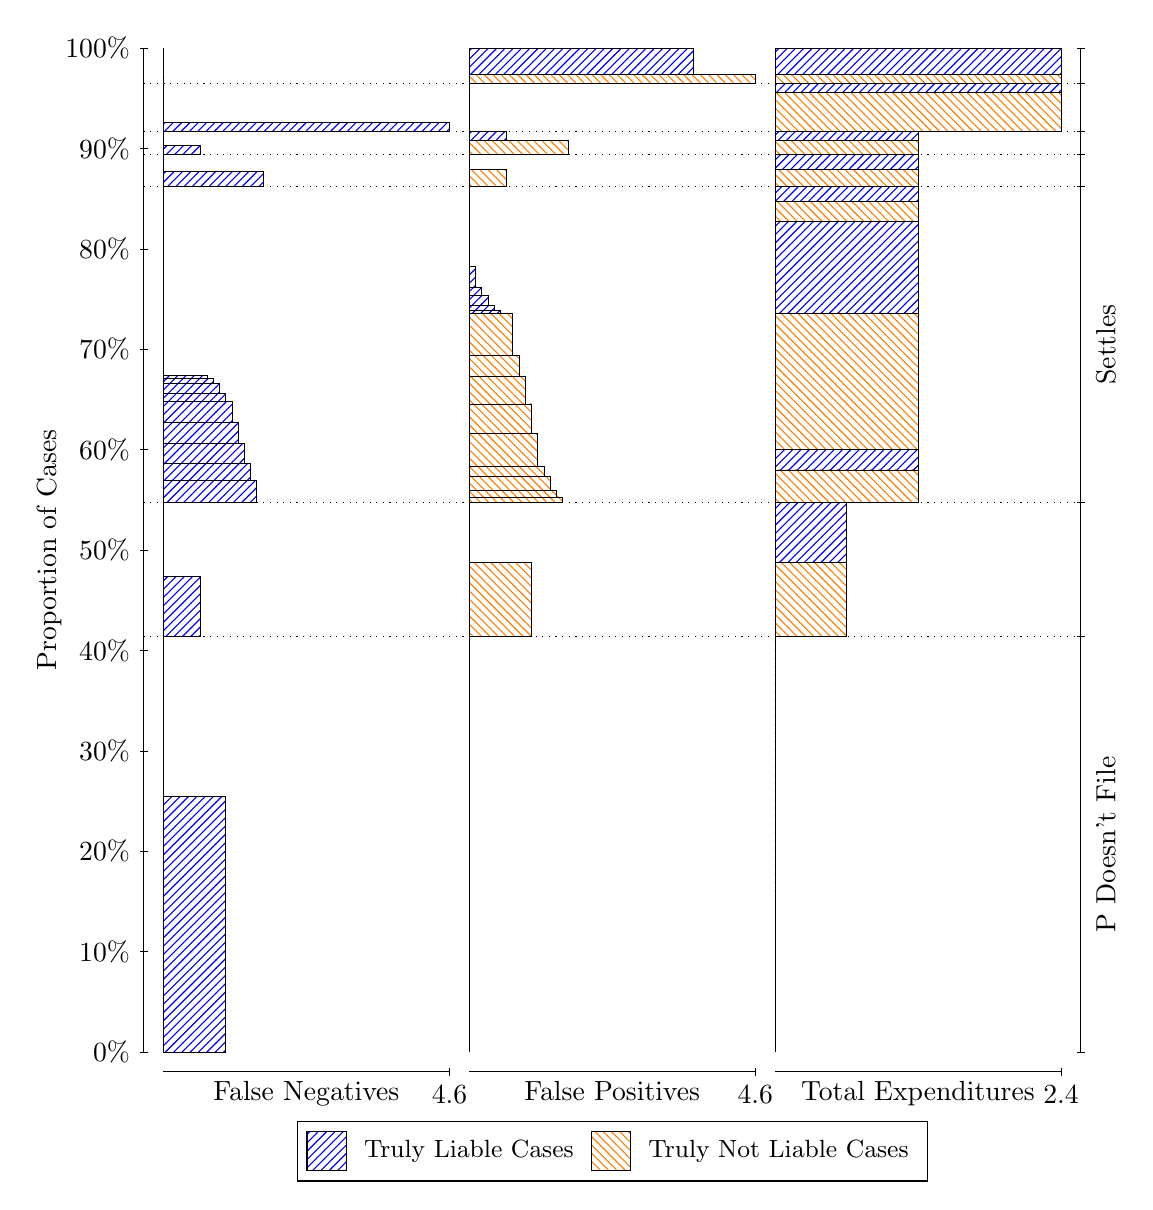
\begin{tikzpicture}
\draw[black, very thin] (1.5,1.75) -- (1.5,14.5);
\node[rotate=90, anchor=center] at (0.3, 8.125) {Proportion of Cases};
\draw[black, very thin] (1.45,1.75) -- (1.55,1.75);
\node[anchor=east] at (1.45, 1.75) {0\%};
\draw[black, very thin] (1.45,3.025) -- (1.55,3.025);
\node[anchor=east] at (1.45, 3.025) {10\%};
\draw[black, very thin] (1.45,4.3) -- (1.55,4.3);
\node[anchor=east] at (1.45, 4.3) {20\%};
\draw[black, very thin] (1.45,5.575) -- (1.55,5.575);
\node[anchor=east] at (1.45, 5.575) {30\%};
\draw[black, very thin] (1.45,6.85) -- (1.55,6.85);
\node[anchor=east] at (1.45, 6.85) {40\%};
\draw[black, very thin] (1.45,8.125) -- (1.55,8.125);
\node[anchor=east] at (1.45, 8.125) {50\%};
\draw[black, very thin] (1.45,9.4) -- (1.55,9.4);
\node[anchor=east] at (1.45, 9.4) {60\%};
\draw[black, very thin] (1.45,10.675) -- (1.55,10.675);
\node[anchor=east] at (1.45, 10.675) {70\%};
\draw[black, very thin] (1.45,11.95) -- (1.55,11.95);
\node[anchor=east] at (1.45, 11.95) {80\%};
\draw[black, very thin] (1.45,13.225) -- (1.55,13.225);
\node[anchor=east] at (1.45, 13.225) {90\%};
\draw[black, very thin] (1.45,14.5) -- (1.55,14.5);
\node[anchor=east] at (1.45, 14.5) {100\%};

\draw[black, very thin] (13.4,1.75) -- (13.4,14.5);
\draw[black, very thin] (13.35,1.75) -- (13.45,1.75);
\node[anchor=west] at (13.35, 1.75) {};
\draw[black, very thin] (13.35,7.0241) -- (13.45,7.0241);
\node[anchor=west] at (13.35, 7.0241) {};
\draw[black, very thin] (13.35,8.7273) -- (13.45,8.7273);
\node[anchor=west] at (13.35, 8.7273) {};
\draw[black, very thin] (13.35,12.743) -- (13.45,12.743);
\node[anchor=west] at (13.35, 12.743) {};
\draw[black, very thin] (13.35,13.148) -- (13.45,13.148);
\node[anchor=west] at (13.35, 13.148) {};
\draw[black, very thin] (13.35,13.44) -- (13.45,13.44);
\node[anchor=west] at (13.35, 13.44) {};
\draw[black, very thin] (13.35,14.05) -- (13.45,14.05);
\node[anchor=west] at (13.35, 14.05) {};
\draw[black, very thin] (13.35,14.5) -- (13.45,14.5);
\node[anchor=west] at (13.35, 14.5) {};

\draw[black, very thin, pattern color=blue, pattern=north east lines] (1.75,1.75) rectangle (2.5399,4.9943);
\draw[black, very thin, pattern color=orange, pattern=north west lines] (1.75,4.9943) rectangle (1.75,7.0241);
\draw[black, very thin, pattern color=blue, pattern=north east lines] (1.75,7.0241) rectangle (2.2239,7.7851);
\draw[black, very thin, pattern color=orange, pattern=north west lines] (1.75,7.7851) rectangle (1.75,8.7273);
\draw[black, very thin, pattern color=blue, pattern=north east lines] (1.75,8.7273) rectangle (2.9348,9.0071);
\draw[black, very thin, pattern color=blue, pattern=north east lines] (1.75,9.0071) rectangle (2.8558,9.2224);
\draw[black, very thin, pattern color=blue, pattern=north east lines] (1.75,9.2224) rectangle (2.7768,9.478);
\draw[black, very thin, pattern color=blue, pattern=north east lines] (1.75,9.478) rectangle (2.6978,9.7483);
\draw[black, very thin, pattern color=blue, pattern=north east lines] (1.75,9.7483) rectangle (2.6188,10.013);
\draw[black, very thin, pattern color=blue, pattern=north east lines] (1.75,10.013) rectangle (2.5399,10.114);
\draw[black, very thin, pattern color=blue, pattern=north east lines] (1.75,10.114) rectangle (2.4609,10.243);
\draw[black, very thin, pattern color=blue, pattern=north east lines] (1.75,10.243) rectangle (2.3819,10.302);
\draw[black, very thin, pattern color=blue, pattern=north east lines] (1.75,10.302) rectangle (2.3029,10.345);
\draw[black, very thin, pattern color=orange, pattern=north west lines] (1.75,10.345) rectangle (1.75,12.743);
\draw[black, very thin, pattern color=blue, pattern=north east lines] (1.75,12.743) rectangle (3.0138,12.933);
\draw[black, very thin, pattern color=orange, pattern=north west lines] (1.75,12.933) rectangle (1.75,13.148);
\draw[black, very thin, pattern color=blue, pattern=north east lines] (1.75,13.148) rectangle (2.2239,13.26);
\draw[black, very thin, pattern color=orange, pattern=north west lines] (1.75,13.26) rectangle (1.75,13.44);
\draw[black, very thin, pattern color=blue, pattern=north east lines] (1.75,13.44) rectangle (5.3833,13.552);
\draw[black, very thin, pattern color=orange, pattern=north west lines] (1.75,13.552) rectangle (1.75,14.05);
\draw[black, very thin, pattern color=orange, pattern=north west lines] (1.75,14.05) rectangle (1.75,14.162);
\draw[black, very thin, pattern color=blue, pattern=north east lines] (1.75,14.162) rectangle (1.75,14.5);
\draw[black, very thin, pattern color=orange, pattern=north west lines] (5.6333,1.75) rectangle (5.6333,3.7797);
\draw[black, very thin, pattern color=blue, pattern=north east lines] (5.6333,3.7797) rectangle (5.6333,7.0241);
\draw[black, very thin, pattern color=orange, pattern=north west lines] (5.6333,7.0241) rectangle (6.4232,7.9662);
\draw[black, very thin, pattern color=blue, pattern=north east lines] (5.6333,7.9662) rectangle (5.6333,8.7273);
\draw[black, very thin, pattern color=orange, pattern=north west lines] (5.6333,8.7273) rectangle (6.8181,8.7993);
\draw[black, very thin, pattern color=orange, pattern=north west lines] (5.6333,8.7993) rectangle (6.7391,8.8854);
\draw[black, very thin, pattern color=orange, pattern=north west lines] (5.6333,8.8854) rectangle (6.6601,9.055);
\draw[black, very thin, pattern color=orange, pattern=north west lines] (5.6333,9.055) rectangle (6.5812,9.1897);
\draw[black, very thin, pattern color=orange, pattern=north west lines] (5.6333,9.1897) rectangle (6.5022,9.6041);
\draw[black, very thin, pattern color=orange, pattern=north west lines] (5.6333,9.6041) rectangle (6.4232,9.9814);
\draw[black, very thin, pattern color=orange, pattern=north west lines] (5.6333,9.9814) rectangle (6.3442,10.33);
\draw[black, very thin, pattern color=orange, pattern=north west lines] (5.6333,10.33) rectangle (6.2652,10.595);
\draw[black, very thin, pattern color=orange, pattern=north west lines] (5.6333,10.595) rectangle (6.1862,11.126);
\draw[black, very thin, pattern color=blue, pattern=north east lines] (5.6333,11.126) rectangle (6.0283,11.168);
\draw[black, very thin, pattern color=blue, pattern=north east lines] (5.6333,11.168) rectangle (5.9493,11.228);
\draw[black, very thin, pattern color=blue, pattern=north east lines] (5.6333,11.228) rectangle (5.8703,11.356);
\draw[black, very thin, pattern color=blue, pattern=north east lines] (5.6333,11.356) rectangle (5.7913,11.457);
\draw[black, very thin, pattern color=blue, pattern=north east lines] (5.6333,11.457) rectangle (5.7123,11.722);
\draw[black, very thin, pattern color=blue, pattern=north east lines] (5.6333,11.722) rectangle (5.6333,12.743);
\draw[black, very thin, pattern color=orange, pattern=north west lines] (5.6333,12.743) rectangle (6.1072,12.958);
\draw[black, very thin, pattern color=blue, pattern=north east lines] (5.6333,12.958) rectangle (5.6333,13.148);
\draw[black, very thin, pattern color=orange, pattern=north west lines] (5.6333,13.148) rectangle (6.8971,13.328);
\draw[black, very thin, pattern color=blue, pattern=north east lines] (5.6333,13.328) rectangle (6.1072,13.44);
\draw[black, very thin, pattern color=orange, pattern=north west lines] (5.6333,13.44) rectangle (5.6333,13.937);
\draw[black, very thin, pattern color=blue, pattern=north east lines] (5.6333,13.937) rectangle (5.6333,14.05);
\draw[black, very thin, pattern color=orange, pattern=north west lines] (5.6333,14.05) rectangle (9.2667,14.162);
\draw[black, very thin, pattern color=blue, pattern=north east lines] (5.6333,14.162) rectangle (8.4768,14.5);
\draw[black, very thin, pattern color=orange, pattern=north west lines] (9.5167,1.75) rectangle (9.5167,3.7797);
\draw[black, very thin, pattern color=blue, pattern=north east lines] (9.5167,3.7797) rectangle (9.5167,7.0241);
\draw[black, very thin, pattern color=orange, pattern=north west lines] (9.5167,7.0241) rectangle (10.425,7.9662);
\draw[black, very thin, pattern color=blue, pattern=north east lines] (9.5167,7.9662) rectangle (10.425,8.7273);
\draw[black, very thin, pattern color=orange, pattern=north west lines] (9.5167,8.7273) rectangle (11.333,9.1417);
\draw[black, very thin, pattern color=blue, pattern=north east lines] (9.5167,9.1417) rectangle (11.333,9.4066);
\draw[black, very thin, pattern color=orange, pattern=north west lines] (9.5167,9.4066) rectangle (11.333,11.135);
\draw[black, very thin, pattern color=blue, pattern=north east lines] (9.5167,11.135) rectangle (11.333,12.3);
\draw[black, very thin, pattern color=orange, pattern=north west lines] (9.5167,12.3) rectangle (11.333,12.556);
\draw[black, very thin, pattern color=blue, pattern=north east lines] (9.5167,12.556) rectangle (11.333,12.743);
\draw[black, very thin, pattern color=orange, pattern=north west lines] (9.5167,12.743) rectangle (11.333,12.958);
\draw[black, very thin, pattern color=blue, pattern=north east lines] (9.5167,12.958) rectangle (11.333,13.148);
\draw[black, very thin, pattern color=orange, pattern=north west lines] (9.5167,13.148) rectangle (11.333,13.328);
\draw[black, very thin, pattern color=blue, pattern=north east lines] (9.5167,13.328) rectangle (11.333,13.44);
\draw[black, very thin, pattern color=orange, pattern=north west lines] (9.5167,13.44) rectangle (13.15,13.937);
\draw[black, very thin, pattern color=blue, pattern=north east lines] (9.5167,13.937) rectangle (13.15,14.05);
\draw[black, very thin, pattern color=orange, pattern=north west lines] (9.5167,14.05) rectangle (13.15,14.162);
\draw[black, very thin, pattern color=blue, pattern=north east lines] (9.5167,14.162) rectangle (13.15,14.5);
\draw[black, dotted] (1.5,7.0241) -- (13.4,7.0241);
\draw[black, dotted] (1.5,8.7273) -- (13.4,8.7273);
\draw[black, dotted] (1.5,12.743) -- (13.4,12.743);
\draw[black, dotted] (1.5,13.148) -- (13.4,13.148);
\draw[black, dotted] (1.5,13.44) -- (13.4,13.44);
\draw[black, dotted] (1.5,14.05) -- (13.4,14.05);
\draw[black, very thin] (1.75,1.5) -- (5.3833,1.5);
\node[anchor=north] at (3.5667, 1.5) {False Negatives};
\draw[black, very thin] (5.3833,1.45) -- (5.3833,1.55);
\node[anchor=north] at (5.3833, 1.45) {4.6};

\draw[black, very thin] (5.6333,1.5) -- (9.2667,1.5);
\node[anchor=north] at (7.45, 1.5) {False Positives};
\draw[black, very thin] (9.2667,1.45) -- (9.2667,1.55);
\node[anchor=north] at (9.2667, 1.45) {4.6};

\draw[black, very thin] (9.5167,1.5) -- (13.15,1.5);
\node[anchor=north] at (11.333, 1.5) {Total Expenditures};
\draw[black, very thin] (13.15,1.45) -- (13.15,1.55);
\node[anchor=north] at (13.15, 1.45) {2.4};

\node[black, centered, rotate=90] at (13.72, 4.387) {P Doesn't File};

\node[black, centered, rotate=90] at (13.72, 10.735) {Settles};





\draw (7.449999999999999,1.5) node[draw=none] (baseCoordinate) {};
\begin{scope}[align=center]
        \matrix[scale=0.5, draw=black, below=0.5cm of baseCoordinate, nodes={draw}, column sep=0.1cm]{
            \node[rectangle, draw, minimum width=0.5cm, minimum height=0.5cm, pattern=north east lines, pattern color=blue] {}; &
            \node[draw=none, font=\small] (B) {Truly Liable Cases}; &
            \node[rectangle, draw, minimum width=0.5cm, minimum height=0.5cm, pattern=north west lines, pattern color=orange] {}; &
            \node[draw=none, font=\small] (B) {Truly Not Liable Cases}; \\
            };
\end{scope}

\end{tikzpicture}
\end{document}